% $XORP: xorp/docs/slides/status_2004_02/xorp.tex,v 1.7 2004/03/05 10:03:46 pavlin Exp $

\documentclass[landscape]{slides}
%\usepackage{ncntrsbk}
\usepackage{epsfig,colordvi}
\frenchspacing

\renewcommand{\baselinestretch}{0.8}
\newcommand{\T}[1]{\center{\PineGreen {#1}}}

\begin{document}

\title{\LARGE \Red{{XORP: An eXtensible Open Router Platform}}}
\author{International Computer Science Institute}
\date{}
\maketitle

% #    #   ####   #####   #####
%  #  #   #    #  #    #  #    #
%   ##    #    #  #    #  #    #
%   ##    #    #  #####   #####
%  #  #   #    #  #   #   #
% #    #   ####   #    #  #
%
%
% #        ####    ####    ####
% #       #    #  #    #  #    #
% #       #    #  #       #    #
% #       #    #  #  ###  #    #
% #       #    #  #    #  #    #
% ######   ####    ####    ####
%
%
% #    #  ######  #####   ######
% #    #  #       #    #  #
% ######  #####   #    #  #####
% #    #  #       #####   #
% #    #  #       #   #   #
% #    #  ######  #    #  ######


%------------------------------------------------------------
\begin{slide}

  \T{The Project}

  \begin{itemize}
  \item Started January 2001
  \item Sponsors
    \begin{itemize}
    \item Intel
    \item National Science Foundation (Award ANI-0129541)
    \item DARPA (Control Plane)
    \end{itemize}
  \end{itemize}

\end{slide}
%------------------------------------------------------------
\begin{slide}

  \T{Objective}

  \begin{itemize}

  \item To replace edge routers with commodity PCs running XORP thus
    enabling innovation and research.
    
    \begin{itemize}

    \item A low end router (350Mhz MIPS processor) performing software
      forwarding. Will only forward 4000 packets per second.

% This 700000 figure is taken from Luigi's measurements where no
% lookups were performed. We could just reduce the number to 100000 or
% qualify the 700000.

    \item A high end PC with dual PCI busses can forward 700000 packets
      per second.

    \end{itemize}

  \end{itemize}

\end{slide}
%------------------------------------------------------------
\begin{slide}

  \T{Deployments}

  \begin{itemize}
  \item PlanetLab testbed for DARPA control plane project (June -
    September 2004)
  \end{itemize}

\end{slide}
%------------------------------------------------------------
\begin{slide}

  \T{Architecture}

  \begin{center}
    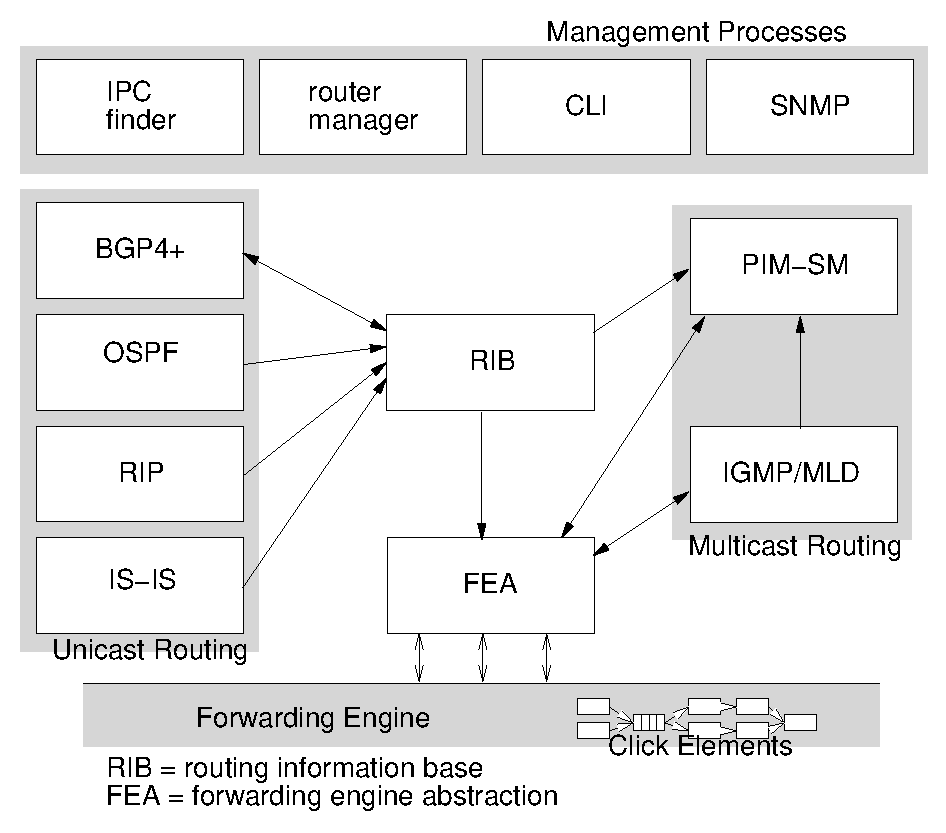
\epsfig{file=../../papers/hotnets_2002_talk/processes3.ps,width=.65\hsize}
  \end{center}

\end{slide}
%------------------------------------------------------------
\begin{slide}

  \T{Design 1}

  \begin{itemize}
  \item Object oriented design in C++.
  \item Each routing protocol is a separate process.
  \item XORP's own interprocess communication (XRLs).
    \begin{itemize}
    \item Processes can be run on any host.
    \item Routing protocols under development can be isolated on
      separate host.
    \item XRLs can be invoked from scripting languages allowing
      easy testing.
    \end{itemize}
  \end{itemize}

\end{slide}
%------------------------------------------------------------
\begin{slide}

  \T{Design 2}

  \begin{itemize}
  \item All routing/forwarding interactions with the operating system
    are performed through the Forwarding Engine Abstraction(FEA).
    \begin{itemize}
    \item Allows distributed or offboard forwarding.
    \item Simplifies porting to new operating systems.
    \item Eases construction of a XORP simulation environment.
    \end{itemize}

  \item The router manager is a fully configurable entity that
    is responsible for process management.
  \end{itemize}

\end{slide}
%------------------------------------------------------------
\begin{slide}

  \T{Extensibility}

  \begin{itemize}
  \item One of the major goals of the project is extensibility.

    \begin{itemize}
    \item Allowing deployment in testbeds such as PlanetLab.
    \item Enabling Research in new or current protocols.
    \end{itemize}

  \end{itemize}

\end{slide}
%------------------------------------------------------------
\begin{slide}

  \T{Suported Platforms}

  \begin{itemize}
  \item FreeBSD
  \item Linux
  \item Mac OS X 10.3 (no FEA)
  \end{itemize}

\end{slide}
%------------------------------------------------------------
\begin{slide}
  \T{Completed Components}

  \begin{itemize}
  \item BGP4+, Full AFI/SAFI support (IPv6 - Multicast), missing route filters
%  \begin{itemize}
%        \item IPv4 tested against Cisco with a full feed
%        \item IPv6 testing against Cisco with full feed in progress.
%        \item IPv6/Multicast against Cisco with full feed in progress.
%  \end{itemize}        

  \item PIM-SM, IGMP (v1 and v2) / MLD (IPv6)  v1
%  \begin{itemize}
%        \item PIM-SM (IPv4) and IGMP - Tested internally in details, and some
%          testing against Cisco.
%        \item MLD - Internal tests only.
%        \item PIM-SM (IPv6) - Internal tests. About to start tests against Cisco.
%  \end{itemize}
  \item RIPv2 and RIPng
%  \begin{itemize}
%        \item RIPv2. Tested with some third party tools (rtquery,
%          ethereal). Not yet tested against another implementation
%        \item RIPng (IPv6). Will be completed tomorrow.
%  \end{itemize}

  \item SNMP using net-snmp
    \begin{itemize}
    \item 
      BGP-4 mib (RFC 1657).
    \end{itemize}
  \end{itemize}

\end{slide}
%------------------------------------------------------------
\begin{slide}

  \T{Expected end of 2004}

  \begin{itemize}
  \item Integration with Click and Planetlab for DARPA control plane project.
  \item Route filters.
  \item Porting of John Moy's OSPF code completed.
  \item IS-IS implementation with basic functionality.
  \end{itemize}

\end{slide}
%------------------------------------------------------------
\begin{slide}

  \T{Possible Future Work}

  \begin{itemize}
  \item Firewall integration (forwarding filters)
  \item Intel network processor (IXP2400) port.
  \item Distributed router.
  \end{itemize}

\end{slide}
%------------------------------------------------------------
\begin{slide}

  \T{Possible Future Research}

  \begin{itemize}
  \item Security (integration with intrusion detection systems)
  \item XORP Simulation environment.
    \begin{itemize}
    \item An environment that allows the development of new protocols
      or features. With the added benefit that the same code will work
      with a real XORP router.
    \end{itemize}
    
  \item Next generation routing protocols.
  \end{itemize}

\end{slide}
%------------------------------------------------------------
\begin{slide}

  \T{Why choose XORP?}

  \begin{itemize}
  \item 1.0 Release Candidate (June 3rd)
  \item Full IPv6 and Multicast support
  \item Designed for extensibility
  \item Ideal research platform
  \item Multiprocess architecture allows construction of distributed routers
  \item Architecture supports high performance network processors
  \end{itemize}

\end{slide}
%------------------------------------------------------------
\begin{slide}

  \T{Summary}

  A XORP based PC router will out perform low end routers. The
  proprietary router market will be opened up enabling innovation and
  research.

  {\huge www.xorp.org}

\end{slide}

\end{document}
